% this file is called up by the header file
% content in this file will be fed into the main document
% ----------------------- paths to graphics ------------------------
\graphicspath{{figures/}}

% ----------------------- contents start here ------------------------

                       
\chapter{Simulation}
\label{chap:simulation}

Given the path loss model established, we can plot the path loss and corresponding channel capacity over distance,
to identify the maximum feasable transmitter-receiver distance $d$. For the following plots, 
a few channel assumptions have been made to reflect a likely 5G network scenario along a highway: 

\begin{center}
\begin{itemize}
    \item Carrier frequency: 28 GHz
    \item Bandwidth: 800 MHz
    \item Transmission Power: 30 dBm
    \item Transmission Gain: 10 dBm
    \item Receiver Gain: 10 dBm
    \item Environment: Rural
\end{itemize}
\end{center}

These assumptions yield the path loss and capacity plots in figure \ref{fig:sim_1} for short distances
(1 - 400m) and figure  \ref{fig:sim_2} for long distances (400 - 2000m). As figure \ref{fig:sim_1} shows, the 
lowest path loss occurs for direct line of sight (LOS) channels, where roughly a 30 dB difference 
between LOS and NLOS cases can be observed in the first 400 meters. Looking at specific factors, such as rainfall, 
it can be obsereved, that even heavy rainfall contributes an insignificant amount of attenuation when compared to NLOS path loss.
Foliage however, 10 m in this case, does produce a significant path loss. \\
Overall, the LOS case yields roughly 100 Mbit/s channel capacity at 200m meters (fig. \ref{fig:sim_1}) and
3 Mbit/s at 1000m of transmitter-receiver distance. \\
Contrary, the NLOS case with foliage decays quickly to 100 Mbit/s of capacity in the first 10 meters. 
The 1 Mbit/s limit is reached after 50 meters and figure \ref{fig:sim_3} shows only a mere 800 bits/s at 400m transmitter-receiver 
distance.\\
One can thus conclude, that for the choosen channel parameters, the NLOS case provides no signifcant data
transfer in ranges over 100 meters. An application as a 5G base station thus seems extremly unlikely in rural 
settings, such as a highway. Solely LOS communication seems feasable. \\
Given a rural highway setting with direct LOS communication between base station and receiver and a medium car density
of 4 cars every 25 meters (both directions), a simultaneous bandwidth of 3.25 Mbits/s could be available for every
participant.

\begin{figure}[htb]
    \begin{center}
        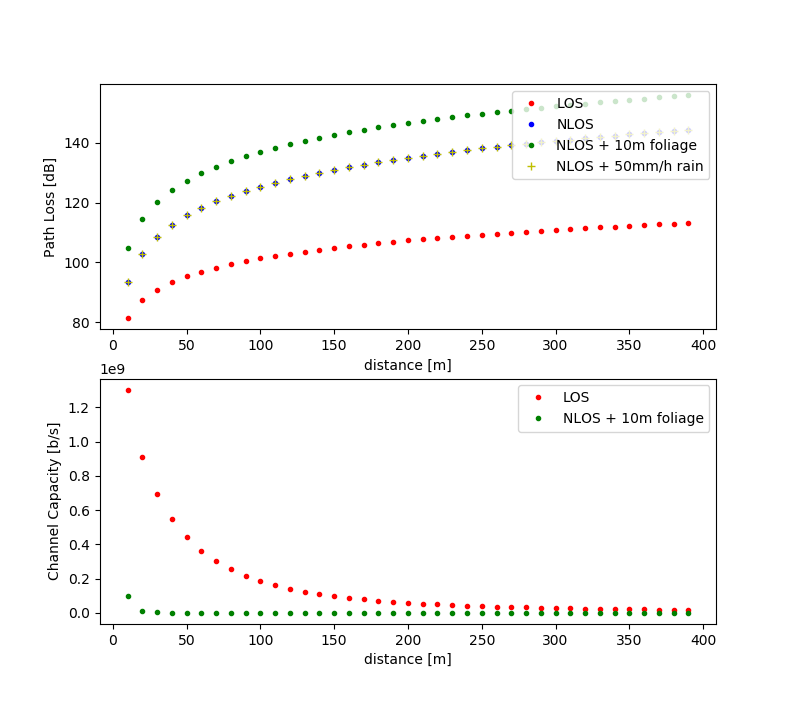
\includegraphics[width=0.9\linewidth]{smba_sim_1}
        \caption{Path loss and channel capacity over 1 to 400 m distance for various environment scenarios, 
        given channel parameter above.}
        \label{fig:sim_1}
    \end{center}
\end{figure}
\begin{figure}[htb]
    \begin{center}
    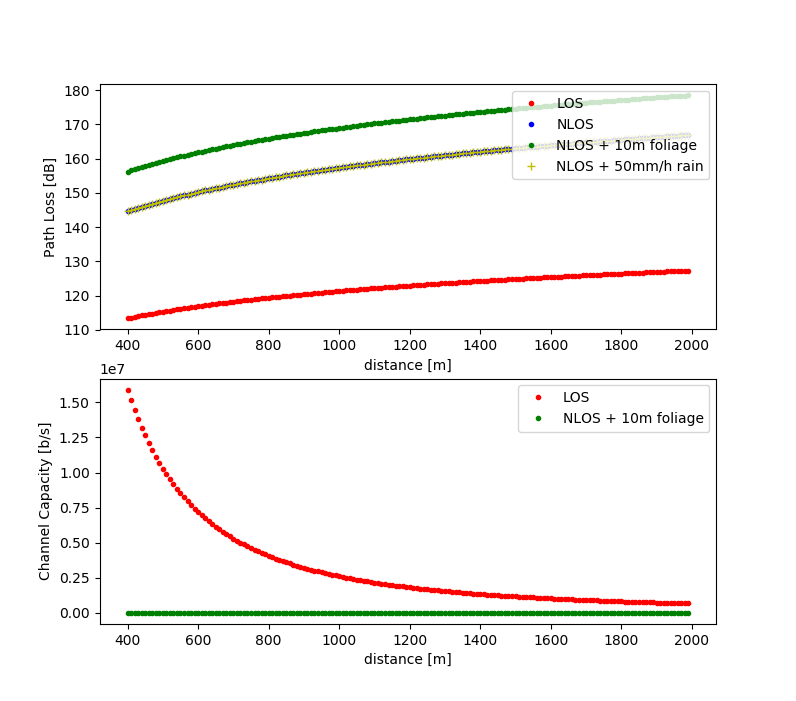
\includegraphics[width=0.9\linewidth]{smba_sim_2}
        \caption{Path loss and channel capacity over 400 to 2000 m distance for various environment scenarios, 
        given channel parameter above.}
        \label{fig:sim_2}
    \end{center}
\end{figure}
\begin{figure}[htb]
    \begin{center}
    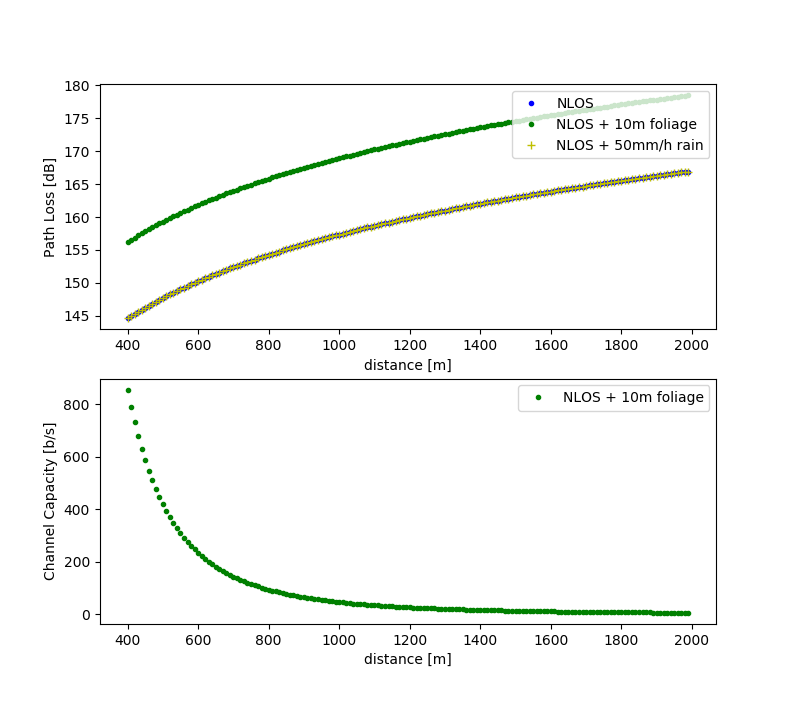
\includegraphics[width=0.9\linewidth]{smba_sim_3}
        \caption{Path loss and channel capacity over 400 to 2000 m distance for NLOS  environment scenarios, 
        given channel parameter above.}
        \label{fig:sim_3}
    \end{center}
\end{figure}

